
%(BEGIN_QUESTION)
% Copyright 2010, Tony R. Kuphaldt, released under the Creative Commons Attribution License (v 1.0)
% This means you may do almost anything with this work of mine, so long as you give me proper credit

The cylindrical displacer in this level transmitter weighs 6.5 pounds (dry) and has a diameter of 1.75 inches.  The process liquid has a specific gravity of 1.25.  The 0\% process liquid level (LRV) is even with the bottom of the displacer, and the URV is even with the top:

$$\includegraphics[width=15.5cm]{i00271x01.eps}$$

Calculate the amount of upward force you would have to apply to the displacer during a ``dry'' calibration to simulate a 50\% full condition.

\vskip 50pt

Calculate the depth of {\it water} the displacer would have to be submerged during a ``wet'' calibration to simulate a 50\% full condition.

\vfil 

\underbar{file i00271}
\eject
%(END_QUESTION)





%(BEGIN_ANSWER)

This is a graded question -- no answers or hints given!

%(END_ANSWER)





%(BEGIN_NOTES)

50\% full, of course, means the displacer will be submerged to the 7.5 inch mark.  For a 1.75 inch diameter displacer and a process liquid with a specific gravity of 1.25, the buoyant force will be:

$$F_{buoyant} = \gamma V$$

$$F_{buoyant} = (1.25)(62.4 \hbox{ lb/ft}^3) \times (7.5 \hbox{ in}) \left(\pi \left({1.75 \over 2} \hbox{ in} \right)^2\right) \left( {1 \hbox{ ft}^3 \over 1728 \hbox{ in}^3} \right) = 0.814 \hbox{ lb}$$

\vskip 10pt

In order to determine the proper water depth to generate this exact same buoyant force, we may use the specific gravity ratio of 1.25 to determine the equivalent depth of submersion.  In other words, we must submerge the displacer in water to a depth that is 1.25 times greater than the depth of this process liquid, since this process liquid exerts 1.25 times more buoyant force than water will at the same depth.

\vskip 10pt

Wet (water) calibration depth = 7.5 $\times$ 1.25 = 9.375 inches

%INDEX% Measurement, level: displacer (buoyancy)

%(END_NOTES)


